\chapter{EEG/ERP Portal}

This chapter describes the motivation behind the creation of EEG/ERP Portal. Crucial technologies and frameworks that have been used in development of EEG/ERP Portal are also described.

\section{About EEG/ERP Portal}

The EEG/ERP Portal is a web-based application which serves to neuroinformatics researchers as a means of managing, sharing and evaluating measured data. The application also comprises advanced featured designed specifically for the needs of EEG/ERP researchers, such as tools for manipulation with EEG signals.


\begin{figure}
	\centering
		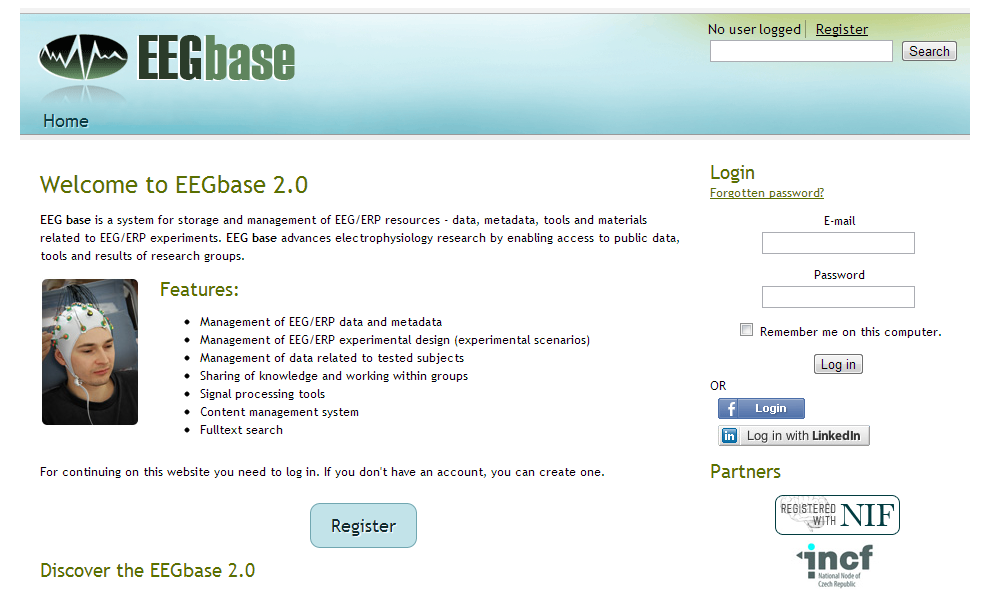
\includegraphics[width=1.00\textwidth]{figures/eegPortal.png}
	\caption{EEG/ERP Portal Welcome Page.}
	\label{fig:eegPortal}
\end{figure}


\subsubsection*{Hibernate}

% Strucne popsat, k cemu je Hibernate a jaky vyuziti ma v portalu. Mozna taky vlozit nejaky schema (z BP?)
Hibernate \cite{Hibernate:Home} is an open-source object-relational mapping framework, whose purpose is to facilitate storage and retrieval of Java domain objects. It is used in EEG/ERP Portal to map its domain model to ...

\subsubsection*{Spring Framework}

% Popsat strucne, jak funguje, jak se vyuziva
The Spring Framework facilitates creating Java-based enterprise applications. It applies a principle called dependency injection which helps to make the classes loosely coupled. The idea of this principle is to let the framework do all necessary wiring of objects, so that the objects can focus on their core responsibilities. 

\subsubsection*{Wicket}

% Popsal v par vetach a uvest, proc se na nej preslo.
... The EEG/ERP Portal's presentation layer is being developed in Wicket by the time of writing this thesis. It is a replacement of JSP pages and Spring MVC. This decision was made due to clearer separation of application logic and markup.
